%%%%%%%%%%%%%%%%%%%%%%%%%%%%%%%%%%%%%%%%
% Compact Laboratory Book
% LaTeX Template
% Version 1.0 (4/6/12)
%
% This template has been downloaded from:
% http://www.LaTeXTemplates.com
%
% Original author:
% Joan Queralt Gil (http://phobos.xtec.cat/jqueralt) using the labbook class by
% Frank Kuster (http://www.ctan.org/tex-archive/macros/latex/contrib/labbook/)
%
% License:
% CC BY-NC-SA 3.0 (http://creativecommons.org/licenses/by-nc-sa/3.0/)
%
% Important note:
% This template requires the labbook.cls file to be in the same directory as the
% .tex file. The labbook.cls file provides the necessary structure to create the
% lab book.
%
% The \lipsum[#] commands throughout this template generate dummy text
% to fill the template out. These commands should all be removed when 
% writing lab book content.
%
% HOW TO USE THIS TEMPLATE 
% Each day in the lab consists of three main things:
%
% 1. LABDAY: The first thing to put is the \labday{} command with a date in 
% curly brackets, this will make a new section showing that you are working
% on a new day.
%
% 2. EXPERIMENT/SUBEXPERIMENT: Next you need to specify what 
% experiment(s) and subexperiment(s) you are working on with a 
% \experiment{} and \subexperiment{} commands with the experiment 
% shorthand in the curly brackets. The experiment shorthand is defined in the 
% 'DEFINITION OF EXPERIMENTS' section below, this means you can 
% say \experiment{pcr} and the actual text written to the PDF will be what 
% you set the 'pcr' experiment to be. If the experiment is a one off, you can 
% just write it in the bracket without creating a shorthand. Note: if you don't 
% want to have an experiment, just leave this out and it won't be printed.
%
% 3. CONTENT: Following the experiment is the content, i.e. what progress 
% you made on the experiment that day.
%
%%%%%%%%%%%%%%%%%%%%%%%%%%%%%%%%%%%%%%%%%

%----------------------------------------------------------------------------------------
%	PACKAGES AND OTHER DOCUMENT CONFIGURATIONS
%----------------------------------------------------------------------------------------                               

% \UseRawInputEncoding

\documentclass[fontsize=11pt, % Document font size
                             paper=letter, % Document paper type
                             %twoside, % Shifts odd pages to the left for easier reading when printed, can be changed to oneside
                             openany, % chapters can start on any page
                             captions=tableheading,
                             index=totoc,
                             hyperref]{labbook}

%\documentclass[idxtotoc,hyperref,openany]{labbook} % 'openany' here removes the
  
\usepackage[bottom=10em]{geometry} % Reduces the whitespace at the bottom of the page so more text can fit

\usepackage[english]{babel} % English language
\usepackage{lipsum} % Used for inserting dummy 'Lorem ipsum' text into the template

\usepackage[utf8]{inputenc} % Uses the utf8 input encoding
\usepackage[T1]{fontenc} % Use 8-bit encoding that has 256 glyphs

\usepackage[osf]{mathpazo} % Palatino as the main font
\linespread{1.05}\selectfont % Palatino needs some extra spacing, here 5% extra
\usepackage[scaled=.88]{beramono} % Bera-Monospace
\usepackage[scaled=.86]{berasans} % Bera Sans-Serif

\usepackage{booktabs,array} % Packages for tables

\usepackage{amsmath} % For typesetting math
\usepackage{graphicx} % Required for including images
\usepackage{etoolbox}
\usepackage[norule]{footmisc} % Removes the horizontal rule from footnotes
\usepackage{lastpage} % Counts the number of pages of the document
\usepackage{float}
\usepackage{fancyvrb}



\usepackage[dvipsnames]{xcolor}  % Allows the definition of hex colors
\usepackage{epstopdf}
\epstopdfsetup{suffix={}}
\definecolor{titleblue}{rgb}{0.16,0.24,0.64} % Custom color for the title on the title page
\definecolor{linkcolor}{rgb}{0,0,0.42} % Custom color for links - dark blue at the moment

\addtokomafont{title}{\Huge\color{titleblue}} % Titles in custom blue color
\addtokomafont{chapter}{\color{OliveGreen}} % Lab dates in olive green
\addtokomafont{section}{\color{Sepia}} % Sections in sepia
\addtokomafont{pagehead}{\normalfont\sffamily\color{gray}} % Header text in gray and sans serif
\addtokomafont{caption}{\footnotesize\itshape} % Small italic font size for captions
\addtokomafont{captionlabel}{\upshape\bfseries} % Bold for caption labels
\addtokomafont{descriptionlabel}{\rmfamily}
\setcapwidth[c]{10cm} % Center align caption text
\setkomafont{footnote}{\sffamily} % Footnotes in sans serif

\deffootnote[4cm]{4cm}{1em}{\textsuperscript{\thefootnotemark}} % Indent footnotes to line up with text

\DeclareFixedFont{\textcap}{T1}{phv}{bx}{n}{1.5cm} % Font for main title: Helvetica 1.5 cm
\DeclareFixedFont{\textaut}{T1}{phv}{bx}{n}{0.8cm} % Font for author name: Helvetica 0.8 cm

\usepackage[nouppercase,headsepline]{scrpage2} % Provides headers and footers configuration
\pagestyle{scrheadings} % Print the headers and footers on all pages
\clearscrheadfoot % Clean old definitions if they exist

\automark[chapter]{chapter}
\ohead{\headmark} % Prints outer header

\setlength{\headheight}{25pt} % Makes the header take up a bit of extra space for aesthetics
\setheadsepline{.4pt} % Creates a thin rule under the header
\addtokomafont{headsepline}{\color{lightgray}} % Colors the rule under the header light gray

\ofoot[\normalfont\normalcolor{\thepage\ |\  \pageref{LastPage}}]{\normalfont\normalcolor{\thepage\ |\  \pageref{LastPage}}} % Creates an outer footer of: "current page | total pages"

% These lines make it so each new lab day directly follows the previous one i.e. does not start on a new page - comment them out to separate lab days on new pages
\makeatletter
\patchcmd{\addchap}{\if@openright\cleardoublepage\else\clearpage\fi}{\par}{}{}
\makeatother
\renewcommand*{\chapterpagestyle}{scrheadings}

% These lines make it so every figure and equation in the document is numbered consecutively rather than restarting at 1 for each lab day - comment them out to remove this behavior
\usepackage{chngcntr}
\counterwithout{figure}{labday}
\counterwithout{equation}{labday}

% Hyperlink configuration
\usepackage[
    pdfauthor={Brian Lauer and Elliot Watkins}, % Your name for the author field in the PDF
    pdftitle={Laboratory Journal}, % PDF title
    pdfsubject={labNotebookSeniorProject1}, % PDF subject
    bookmarksopen=true,
    linktocpage=true,
    urlcolor=linkcolor, % Color of URLs
    citecolor=linkcolor, % Color of citations
    linkcolor=linkcolor, % Color of links to other pages/figures
    backref=page,
    pdfpagelabels=true,
    plainpages=false,
    colorlinks=true, % Turn off all coloring by changing this to false
    bookmarks=true,
    pdfview=FitB]{hyperref}

\usepackage[stretch=10]{microtype} % Slightly tweak font spacing for aesthetics

\usepackage[framed,numbered,autolinebreaks,useliterate]{mcode}
\usepackage{todonotes}

%\setlength\parindent{0pt} % Uncomment to remove all indentation from paragraphs

%----------------------------------------------------------------------------------------
%	DEFINITION OF EXPERIMENTS
%----------------------------------------------------------------------------------------

% Template: \newexperiment{<abbrev>}[<short form>]{<long form>}
% <abbrev> is the reference to use later in the .tex file in \experiment{}, the <short form> is only used in the table of contents and running title - it is optional, <long form> is what is printed in the lab book itself

\newexperiment{example}[Example experiment]{This is an example experiment}
\newexperiment{example2}[Example experiment 2]{This is another example experiment}
\newexperiment{example3}[Example experiment 3]{This is yet another example experiment}

\newsubexperiment{subexp_example}[Example sub-experiment]{This is an example sub-experiment}
\newsubexperiment{subexp_example2}[Example sub-experiment 2]{This is another example sub-experiment}
\newsubexperiment{subexp_example3}[Example sub-experiment 3]{This is yet another example sub-experiment}

%----------------------------------------------------------------------------------------
\newcommand{\HRule}{\rule{\linewidth}{0.5mm}} % Command to make the lines in the title page

\setlength\parindent{0pt} % Removes all indentation from paragraphs

\begin{document}

%----------------------------------------------------------------------------------------
%	TITLE PAGE
%----------------------------------------------------------------------------------------
%\frontmatter % Use Roman numerals for page numbers

%\begin{center}

%

\title{
\begin{center}
\href{http://www.bradley.edu}{
\includegraphics[height=0.5in]{figs/logoBU1-Print}}
\vskip10pt
\HRule \\[0.4cm]
{\Huge \bfseries Laboratory Notebook \\[0.5cm] \Large Development of an Intelligent Building Energy Management System}\\[0.4cm] % Degree
\HRule \\[1.5cm]
\end{center}
}
\author{\Huge Brian Lauer and \Huge Elliot Watkins \\ \\\Large blauer@mail.bradley.edu, ejwatkins@mail.bradley.edu} % Your name and email address
\date{Beginning September 14, 2020} % Beginning date
\maketitle

%\maketitle % Title page

\printindex
\tableofcontents % Table of contents
\newpage % Start lab look on a new page

\begin{addmargin}[0cm]{0cm} % Makes the text width much shorter for a compact look

\pagestyle{scrheadings} % Begin using headers

%----------------------------------------------------------------------------------------
%	LAB BOOK CONTENTS
%----------------------------------------------------------------------------------------
r. 
\labday{Monday, September 14, 2020}

\experiment{Meeting Minutes}
BL \\
Today, in the meeting with Dr. Miah, we kicked off the project involving development of a building enery management platform. A Github repository was created for the project which will also be paired with a corresponding Google Drive titled "seniorProject1-2020-21". On Tuesdays and Thursdays, we will have lab time from 8am to 11am and weekly meetings with the advisor from 4pm to 5pm on Mondays this semester. The lab times are devoted specifically for work rather than research or documentation. Before coming to lab, work must be cut out for both of us.

\experiment{Homework}
BL\\
This document was created and pushed to the Github repository for both of us to use. For better portability, one of the laptops previously used for research on this project was wiped clean and LUbuntu was installed. As of now, most of the code developed for the platform was done on a desktop PC dual-booted with Ubuntu Linux and Windows 10. To be able to move between lab and home easily, a more ideal situation is to use a dedicated laptop with Linux installed. Because the USB drive used to install Linux was previously formatted with Ubuntu 18.04, the diskpart utility was used with the following commands:
\begin{Verbatim}
select disk 1
clean 
create partition primary
format quick
\end{Verbatim}
The Startup Disk Creator GUI program on Linux was utilized to flash the LUbuntu 64-bit desktop iso file on to the USB-thumb drive. The commands \texttt{sudo apt-get update} and \texttt{sudo apt-get upgrade} were run on the laptop to perform necessary upgrades and updates. Lastly, \texttt{sudo apt-get install git} was used to install git. Another package installed was \texttt{textlive-full} to compile latex with all the necessary packages.
%-------------------------------------------

\labday{Monday, September 21, 2020}

\experiment{Meeting Minutes}
BL\\
In the meeting with Dr. Miah, Dr. Miah pointed out that templates are available in the Google Drive for the lab notebook and other deliverables which we did not realize. In the System Level Requirements document (the first deliverable) we must replace the current block diagram with the drawing of the house connected to a microgrid. Inside, the home will be a block of the BEMS core which will connect to various IoT devices in the building. The controllable loads in the building including devices like lights, appliances (including dishwashers, washing machines), and smart plugs. Examples of uncontrollable loads include desktop PCs, laptops, thermistors, and microwaves. In a potential future research project, connectivity with a microgrid may be possible, so powerlines representing the main grid will be connecting the house to a microgrid through a PCC (Point of Common Coupling). In the current version of the diagram, the file is simply too large as it contains many images from the Internet. This will be redrawn in inkscape with custom figures to reduce the file size.
\smallbreak\noindent
The final outcome of the project will be
\begin{itemize}
\item Laptop running in the IoT lab or office
\item 2-3 devices in office/lab can be controlled succesfully
\item System should recognize the devices immediately upon connection to the network
\item Algorithm implemented to help improve energy efficiency
\end{itemize}
As a part of the first deliverable, three modes of operation will be declared including
\begin{itemize}
\item Device search mode
\item Device operation mode
\item Third mode to be determined
\end{itemize}
The sections of the deliverable will be
\begin{itemize}
\item Problem Statement
\item System Architecture
\item Block Diagram
\item Modes of Operation
\end{itemize}
Another point brought up is whether an energy efficient algorithm should be included in the software. Dr. Miah said yes. This will possibly help to boost the complexity of the project and improve the usefuleness of the platform. This algorithm will have to be determined.
\smallbreak\noindent
As of today, we should both be writing code on Tuesdays and Thursdays or possibly on our own, and we can both use code written for the research project. The split should be 50/50 so a Gantt chart will need to be made. 
%--------------------------------------------------------------------c--------------------

\labday{Tuesday, September 22, 2020}

\experiment{Lab work}

BL\\
Elliot and I met over Zoom to work on getting a new Github repo setup for the senior project code specifically. Although Dr. Miah mentioned in the meeting that the code should be on Github, we simply will periodically upload the zipped Github project to the Drive to the implementation/ folder. I copied over the files from the research to the new Github repo cloned locally on my Linux laptop. After running the \texttt{install.sh} script, the installation failed as the Linux laptop I am using is running Python3.5 rather than Python3.6 which is required for f-string support. An example of a line that failed is shown in the figure below:
\begin{figure}[H]
\centering
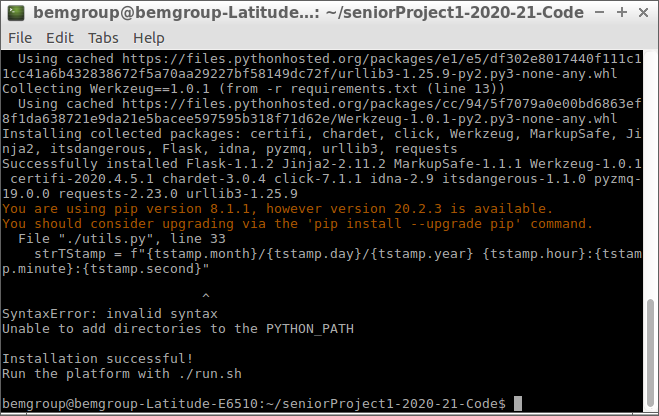
\includegraphics[scale=0.6]{figs/img/installSyntaxError}
\caption{f string error in \texttt{utils.py}}
\end{figure}
A simple solution to this problem was simply using string concatenation:
\begin{Verbatim}
strTStamp = str(tstamp.month) + "/" + str(tstamp.day) + "/" + str(tstamp.year) + " "
strTStamp += str(tstamp.hour) + ":" + str(tstamp.minute) + ":" + str(tstamp.second)
\end{Verbatim}
Further changes were made in the \texttt{ControlAgent.py} and \texttt{DiscoveryAgent.py} files. In particular, the line in \texttt{subscribe} to connect to the server acting as the central exchange to process publish/subscribe messages between the web server backend and agents listening for subscriptions was altered to support string concatenation. After these alterations to the source code were made, the platform was succesfully started. However, it is clear that no messages published to the server were received by both either the \texttt{ControlAgent} or \texttt{DiscoveryAgent} which will need to be debugged in the next lab or possilby before. This is evident as the terminals showing the debug output of each agent not indicating any messages received. Messages should be published via the publish function in the file \texttt{PROJECT\_DIR/WebServer/pubsub.py}. All these problems must be fixed to allow the ActiveDevices page to discover and connect to devices.
\end{addmargin}
%--------------------------------------------------------------------c--------------------

\labday{Thursday, September 24, 2020}
BL\\
Today, I debugged some of the problems with the \texttt{ControlAgent} agent not receiving messages. The agent was run in isolation and tested with the publish function in the \texttt{pubsub.py} file. The agent was able to successfully receive messages. However, this was not tested while the platform was running which will need to be done in the next lab session.

I (Elliot) started to create a device driver for the BeagleBone Blue based off of the WeMo Switch driver. In doing so, I also started researching ways to control individual pins via wifi, starting with the GPIO.

\labday{Monday, September 28, 2020}

\experiment{Meeting Minutes}
EW\\

\textbf{Agenda:}

How to auto-detect devices on the network (interrupt or polling)? We were thinking of constantly pinging the network for supported devices in an infinite loop. Is there a way for a device to send a request to the server once it has joined the network?

We would like to add support for a smart power meter that can connect to WiFi,
so power data for the entire building/house can be shown in the UI. What would
you recommend in terms of a cost-effective solution? I found a device called the
Sense Energy Monitor that can send data over wifi to an mobile or web app that
comes with the device. The device itself connects to the electrical panel of a
house. However, it is quite expensive at a price of 299 dollars.

Does the platform still need to be agent-based like BEMOSS? 

\textbf{Discussion:} For auto-detecting, we need to research how to create an
interrupt. IF that turns out to be impossible, we will try to replicate Windows
trying to find bluetooth devices. It will be a poling process that is explicitly
demanded by the user.

MATLAB can be used to measure power usage. Simscape is an addon that includes a
power sensor module. After checking online, we also discovered it is possible to
connect MATLAB to a website and transfer data. With this, we should be able to
plot power usage on the UI.

FInally, Dr. Miah informed us that the project will indeed be agent-based.

Helpful Links:

https://drive.google.com/file/d/1jx7SldW3zNLdA5WBNl89LUBIK0KQuEMl/view?usp=sharing
https://www.codeguru.com/
https://smile.amazon.com/Bluetooth-Voltmeter-Multimeter-Resistance-Impedance/dp/B07PZRSYXD/

\labday{Tuesday, September 29, 2020}

\experiment{Lab work}
BL\\
Today, work was done on getting the linux laptop connected to the "AERO" network in the senior project lab, so that experiments can be done properly with the WeMo Switch and eventually Beaglebone Blue. Because this was not working, Elliot set up a hotspot on his laptop which was tethered through BUSecure. Secondly, Elliot paired the WeMo Switch with the WiFi network in the lab with his phone as I did not remember the password to my WeMo account, so a new one was made. A couple of bugs were still present in the current version of the software. One of them was causing the \texttt{ControlAgent} to crash everytime a publish message was attempted to be sent through interprocess communication. We found the problem was due to the following error
\begin{Verbatim}
can't convert type 'dict' to 'str' implicitly
\end{Verbatim} 
This was fixed by using \texttt{json.dumps} in the \texttt{pubsub.publish} function. At the end of the lab session, we were able to succesfully toggle the WeMo Switch on and off through our platform. One of the things Elliot pointed out was the fact that the checkbox toggle button for turning the device on and off is not set to the proper position when the page is loaded as it is always in the off position. We decided this feature will need to be added soon as it had not been added.

\labday{Thursday, October 1, 2020}

\experiment{Lab work}
BL\\
We decided to write down the trace of commands/function calls that occur from the top layer (UI layer) all the way down to the bottom layer (device API layer) to turn on/off the Switch:
\begin{itemize}
\item Main active devices page: \texttt{PROJECT\_DIR/WebServer/templates/active\_devices.html}
\item JS code running on \texttt{active\_device.js} calls \texttt{\$.ajax()} which sends an AJAX request to the url '/active\_devices/ajax/setDeviceStatus'
\item Sending a POST request to URL '/active\_devices/ajax/setDeviceStatus' calls sendDeviceStatusToControlAgent()
\item In subscribe of \texttt{PROJECT\_DIR/AgentPlatform/ControlAgent.py} a call to processMethod() occurs which calls setDeviceStatus()
\item setDeviceStatus() calls \texttt{WeMoAPI.setState}
\item \texttt{PROJECT\_DIR/DeviceDrivers/WeMoAPI.py} setState() function sends an XML SOAP request over HTTP to the WeMo Switch
\end{itemize}
In order to display the correct device status on the web server via the \texttt{getDeviceStatus()} method in the \texttt{ControlAgent} class:
\begin{itemize}
\item \texttt{getState} will retrieve the status using XML SOAP requests
\item \texttt{renderActiveDevices()} will be called in \texttt{active\_devices.py}. We would like to eventually poll for a state change (Not necessarily this function). Also, we want to use the most recent timeseries data from a table.
\item First we will need to use \texttt{getState()}, but eventually we want to use a data table. Also, we need to research interrupts. 
\end{itemize}
I suggested installing the Cassandra database in the software as a first step towards getting the status updated on the web page as it can store time series data easily. The instructions for install Cassandra are listed below taken from \footnote{\url{https://cassandra.apache.org/download/}}
\begin{enumerate}
\item \texttt{echo "deb https://downloads.apache.org/cassandra/debian 311x main" | sudo tee -a /etc/apt/sources.list.d/cassandra}
\item \texttt{curl https://downloads.apache.org/cassandra/KEYS | sudo apt-key add -}
\item \texttt{sudo apt-get update}
\end{enumerate}
We encountered the following error which was documented on the site
\begin{verbatim}
GPG error: http://www.apache.org 311x InRelease: 
The following signatures couldn't be verified 
because the public key is not available: NO\_PUBKEY: E91...
\end{verbatim}
The PUBKEY is extracted from the error message itself and must be added with 
\texttt{sudo apt-key adv --keyserver pool.sks-keyservers.net --recv-key E91..}
\medbreak\noindent
Lastly the software was installed with \texttt{sudo apt-get install cassandra}. To interface with the software with Python, we decided to use the DataStax Python driver for Apache Cassandra. It was installed with the following commands
\begin{enumerate}
\item source venv/bin/activate
\item pip3 install cassandra-driver
\end{enumerate}

\labday{Monday, October 5, 2020}
\experiment{Meeting}
BL\\
\textbf{Agenda:}
\begin{itemize}
\item What is a reliable and efficient way to obtain the status of the WeMo and update the checkbox on the web page? This is needed in case someone turns the WeMo on and off manually.
\item Is a Gantt chart required for the first deliverable?
\item Could you review what we have written so far for the first deliverable?
\item We are considering integrating the DC motor with the software through the BeagleBone Blue. As an extension from the project in 2019 would we be able to add a speed control algorithm to use PWM to control motor speed? If so, should we develop our own or use the one from your mechatronics textbook?
\end{itemize}

\experiment{Meeting}
BL\\
\textbf{Minutes:}
\begin{itemize}
\item We should use an Interrupt Service Routine to get device status from Wemo Switch. This will be used to update the status being displayed on the web server. 
\item We will not be using a Gantt chart.
\item If we want to implement the DC motor, we have to come up with a useful application. The shaft must be connected to a load. We are thinking of driving a fan which could realistically be used to control a fan possibly a CPU heatsink fan. It does not matter if we use Dr. Miah's control algorithm or our own.
\item Our current issue is: the Wemo switch fails to turn on/off from the application if someone turns it on/off manually. For
\end{itemize}

\labday{Tuesday, October 6, 2020}
\experiment{Lab work}
BL\\
Today, Elliot and I worked on ways of possibly implementing an interrupt whenever the WeMo Switch is turned on or off. Various blogs on interrupts in Python3 were found regarding KeyboardInterrupts and GPIO with the Raspberry Pi. It may not be possible to cause the Switch to generate an interrupt signal on its own as this may not be built into the firmware of the device. Initially some problems were encountered as a problem was encountered in the file \texttt{PROJECT\_DIR/WebServer/static/js/apps/active\_device.js} as the Javascript object named \texttt{evt} was not passed as a parameter to the callback function for the input checkbox event listener. This was then used to call
\begin{Verbatim}
evt.preventDefault();
\end{Verbatim}
which according to the Jquery documentation cancels the default navigation of the click. This is not necessarily needed as it runs properly without the method call. Work was done on implementing the feature to update the checkbox position whenever the DOM is ready. One of the problems that needs to be solved is obtaining the data from the web server after sending a AJAX GET request. This will be done by receiving a JSON object in the response to the AJAX request. According the jQuery documentation\footnote{\url{https://api.jquery.com/jquery.ajax/}}, one of the optional arguments to be passed is the \texttt{success} parameter which can hold the arguments
\begin{itemize}
\item data
\item status
\item settings
\end{itemize}

\labday{Thursday, October 8, 2020}
\experiment{Lab work}
BL and EW\\
One of the problems we faced into today's lab session was the Switch's port number incrementing by 1. Yesterday, the port number was 49154 and today it is 49155. We'll have to determine why this is happening.
We are also trying to improve the getDeviceStatus() function to get both the id of the WeMo and the powerstate. A solution to this problem is using a list nested in a dictionary along with a key value pair for the id of the device. One of the feaures of javascript that we do not know to implement is how to set the checkbox position with javascript.

\labday{Monday, October 12, 2020}
\experiment{Meeting}
BL\\
\textbf{Agenda}
\begin{itemize}
\item Go over current presentation
\item Schedule an appointment for presentation
\item Additional ECE faculty member for presentation
\end{itemize}

\experiment{Meeting}
EW\\
\textbf{Minutes:}
\begin{itemize}
\item We should put the Deliverables into a folder for Deliverables in the Docs repo.
\item For the introduction to the presentation, we should have photos/animations in addition to text (Columns).
\item Start with diagrams, then have text to explain more details.
\item The diagram with the BeagleBone Blue - it should just be called an embedded computer. Also, no black blocks; add more color.
\item Text and Diagrams should be directly related - Have 1 slide for each major part of each diagram.
\item When making a presentation, keep in mind that we need to sell this to a third party who will not understand everything.
\item In Figure 2, label the signals going to and from the BEMS Core.
\item Start with minimum requirements, and then talk about exceeding that.
\end{itemize}

\labday{Tuesday, October 13, 2020}
EW\\
\experiment{Lab work}
Brian and I tried to get the refresh button on the "active devices" page to reload the check box for the WeMo switch. This task is proving to be more challenging than we thought. Neither of us has much experience with JavaScript. We need to learn how to access each button and their properties in active\_device.js if we want this feature to work.

\labday{Thursday, October 15, 2020}
EW\\
\experiment{Lab work} Today, the Aero router was missing from the lab. We
instead used my Windows laptop as a hotspot to connect to the Wemo. Once we got
connected, we continued with the task of updating the check box on the active
devices page with the current Wemo status. At the beginning of this session,
refreshing the check box would turn the Wemo on or off instead of just changing
the check box. By 9:22 AM, we were able to refresh the status of the check box
on the active devices page with the actual state of the Wemo switch. I took a
short video of our progress with the Wemo Switch; that needs to be uploaded to
the Deliverables folder of the Docs repo. Next, we decided to start implementing
the Apache Cassandra database. This will lead us into the next feature for the
Wemo: recording power usage. Our plan:

\begin{itemize}
\item Set up the database
	\begin{itemize}
	\item The Cassandra database needs to be set up outside of python, then it can be accessed
	\item We believe we can automate the set up process with a shell script that can be run from python
	\end{itemize}
\item Implement a function to write data to it 
\item Implement a function to read data back from the database
\item Implement a function to display data on the active devices page
\item Figure out a way to plot a graph of power usage with matplotlib in python
\end{itemize}

\labday{Monday, October 19, 2020}
\experiment{Meeting minutes}
BL\\
Agenda:
\begin{itemize}
\item System level requirements pres
\item Changes to be made to the sys level requirements draft
\item Should Elliot and I work together on the same features (pair programming) or work separately on different tasks?
\item Should we have a well defined schedule of what features we would like to work for the rest of senior project?
\end{itemize}

Minutes:
\begin{itemize}
\item We should list all the features found in BEMOSS or another BEMS platforms and explain how ours is different. We need to gather some standard features that people have used in similar projects. Find at least 5 other platforms. Use library resources and contact Dr. Miah if we can't get access to a source.
\item I (Elliot) will start implementing support for the beaglebone blue and Brian will work on implementing additional features (right now that is the Apache Cassandra Database and power recording).
\end{itemize}

\labday{Tuesday, October 20, 2020}
\experiment{Lab work}
EW\\
Today, I started looking into running python files on the BeagleBone Blue. I installed the Adafruit library: https://pypi.org/project/Adafruit-BBIO/ and was able to run a simple program to flash the on-board LEDs. However, Dr. Miah mentioned that I should look into the rcpy library as an alternative. After settling on a control library, I need to figure out how to connect to the BeagleBone Blue from the platform.
Dr. Miah also reminded us both to start looking into standard features found in other energy management systems similar to BEMS.
\medbreak\noindent
BL\\
I worked on adding calls to the various cassandra library methods and class constructors to interact with the Cassandra database. In the Discovery agent, I added a query to create a new table for each device when it is discovered by the discovery agent in the \texttt{setDeviceToActive} method. Each table will have fields
\begin{itemize}
\item id text
\item power double
\item status text
\item tstamp timestamp
\end{itemize}
for now. However, this will likely need to be changed when new devices are added. Secondly, another query execution call was added to the method \texttt{periodicQueryBehavior} in the \texttt{ControlAgent} which will add a new entry to a given device table every 10 seconds inside a separate thread from the main program. In order to initialize the database, a keyspace was created titled "bemstimeseries" which will need to be added to the database when the platform is installed. This likely be added to the \texttt{install.sh} script. The last task I worked on was installing matplotlib which gave me trouble as python3.5 is installed on the LUbuntu laptop running the server. However, this python package requires Python3.6 and later. I will need to work on figuring out how to update python on the laptop if possible. 

\labday{Thursday, October 22, 2020}
\experiment{Lab work}
BL\\
I decided to try just installing matplotlib and all the necessary dependencies like numpy with older versions supported by python3.5. The following dependencies and their corresponding versions are required for python3.5
\begin{itemize}
\item matplotlib==1.5.1
\item numpy==1.11.0
\item dateutil==2.4.2
\item pytz==2014.10
\end{itemize}
Another problem was encountered when attempting to install the dateutil python3 package as a messaged was displayed that python3.5 reached the end of its life on September 13, 2020. A solution to this problem I will try to implement is installing the latest version of Lubuntu 20.04 LTS. Dr. Miah approved this.
\medbreak\noindent
The next task is to determine where to create a new keyspace in the cassandra table. I added this in the \texttt{run.sh} file for now but may make more sense to place in the \texttt{install.sh} file. Next I worked on inspecting the keyspace for new tables when a new device is discovered. Unfortunately, no new tables were showing up after the \texttt{DiscoveryAgent} did its work in the \texttt{setDeviceToActive} method. The CQL query:
\begin{Verbatim}
SELECT * FROM system_schema.tables WHERE keyspace_name = 'bemstimeseries';
\end{Verbatim}
should list all the table information in the 'bemstimeseries' keyspace. The next logical step is to run the query in the \texttt{setDeviceToActive} method which will create a table for the device. In the \texttt{cqlsh} command line program, I ran into the exception
\begin{Verbatim}
InvalidRequest: Error from server: code=2200 [Invalid query] 
message="No PRIMARY KEY specifed (exactly one required)"
\end{Verbatim}
This error makes sense as no primary key was supplied in the CREATE TABLE command. A second error was encountered after adding in a primary key:
\begin{Verbatim}
SyntaxException: line 1:59 no viable alternative at input 
'PRIMARY_KEY' (... EXISTS bemstimeseries.device1 (id [UUID] PRIMARY_KEY...)
\end{Verbatim}
After executing the query 
\begin{Verbatim}
CREATE TABLE IF NOT EXISTS bemstimeseries.wemo 
(id UUID PRIMARY_KEY, power double, status text, tstamp timestamp);
\end{Verbatim}

EW\\
I have made some progress on the Beaglebone API. It is possible to connect to the beaglebone via python socket programming and send commands. This will be the basis for controlling the beaglebone from the platform. At the end of lab today, I was having trouble running the program to turn on the on-board LEDs. I need to figure out why that is not working and then add more functions to better control the LEDs. Eventually, this will be integrated into the platform and the discovery/control agents will be used to access and control beaglebones. We will also need wires to connect to the motor drivers.

\labday{Monday, October 26, 2020}
\experiment{Meeting}
EW\\
\textbf{Agenda}
\begin{itemize}
\item Links to IEEE articles on BEMS we don't have access to: 
	\begin{itemize}
	\item https://ieeexplore-ieee-org.ezproxy.bradley.edu/document/6852647
	\item https://ieeexplore-ieee-org.ezproxy.bradley.edu/document/8494012
	\item https://ieeexplore.ieee.org/document/8246800
	\end{itemize}
Other sources with features for BEMS:
	\begin{itemize}
	\item https://greencoast.org/building-energy-management-systems/
	\end{itemize}

\item Go over progress on BeagleBone Blue API (Elliot)

\end{itemize}

BL\\
\textbf{Other links}
\begin{itemize}
\item https://ieeexplore.ieee.org/document/8403212
\item https://www.mdpi.com/2071-1050/9/2/264/pdf-vor
\item https://www.mdpi.com/2079-9292/8/7/763 - LoBEMS - LoRa Building and Energy Management System	
\end{itemize}
From third link (LoRa BEMS), some of the features added to their platform are
\begin{itemize}
\item LoRa support
\item A/C automation
\item Plot of A/C usage
\item air quality monitoring
\item If This Then That support - BEMS was tested at a school, parents were notified when the air quality was too low
\item Sensors with SOC's, powered by batteries, using the LoRa communication interface monitored temperature, humidity, luminosity, and air quality
\end{itemize}


\textbf{Minutes}
\begin{itemize}
\item Beaglebone API connection is valid. Need to continue building functionality.
\item Cassandra Database is a valid option for storing data. We will continue working with that. Brian should try Setting the primary key to "device ID."
\item The final paper that Brian found is an excellent source to reference, we will be reading this in the near future.
\item Dr. Miah will look into the papers that Elliot found to see if they are good sources to use.
\end{itemize}

\labday{Thursday, October 22, 2020}
\experiment{Lab work}
EW\\
Today, I made some more progress with the socket connection to the BBB (beaglebone blue). I wrote a couple a functions in a file called LED.py to control the LEDs. Then, I ran a socket server on my laptop and a client on the BBB that could call those functions in LED.py. This was a major milestone because it proved that programs can be run on the BBB from a laptop connected over wifi. My next task will be altering the server/client relationship to be more robust. Right now, it has to go back and forth between the server and client, I would like to be able to send multiple messages to the client and vice versa.

\labday{Thursday, October 29, 2020}
BL\\
Work was continued on getting the data logging feature implemented for the WeMo Switch. I came across this problem:
\begin{Verbatim}
Traceback (most recent call last):
  File "/usr/lib/python3.8/threading.py", line 932, in _bootstrap_inner
    self.run()
  File "/usr/lib/python3.8/threading.py", line 870, in run
    self._target(*self._args, **self._kwargs)
TypeError: periodicQueryBehavior() argument after * must be an iterable, not int
\end{Verbatim}
I decided to try and run the ControlAgent to debug the problem with an int getting sent to the \texttt{periodicQueryBehavior} rather than an iterable object like a list or string.
\medbreak\noindent
Further problems were encountered when multiple WeMo switches were appearing on the active devices page. Some of the problems were still being reported in the terminals. The next step is to determine how to properly add a timestamp to a database entry. Some of the problems were fixed with adding entries to the device table for the Switch. However, when adding a timestamp, the following was added by using the cql call \texttt{toTimeStamp(now())}
\begin{Verbatim}
2020-10-29 16:42:28.166000+0000
\end{Verbatim}
The current time in the lab was 11:42 am meaning the timezone must be configured. Research will have to be done on this topic. First, a problem with the current columns in the table is the presence of an id column which is actually defined in the name of the table. The id column will be removed. However, a primary key is required. Originally this was set as the id column but will be changed to the timestamp column.

EW\\
Continued working on the server and client files for connecting to the BBB. I created 2 new files called new\_server.py and new\_client.py. new\_server.py uses object-oriented programming to create a server and then run specific functions. The goal here is to produce several functions for controlling the BBB that the BEMS core will be able to call instead of having the user manually type commands in a terminal.

\labday{November 2, 2020}
\experiment{Meeting}
BL\\
\textbf{Agenda}
\begin{itemize}
\item May we use a process control algorithm like Model Predictive Control or Linear Quadratic Regulator to simulate control of building temperature? I was thinking we could have some sort of HVAC model that is able to communicate with our BEMS. We could try to predict the appropriate amount of heat to apply to the building depending on the outside temperature. I found an article listed in our proposal regarding this method. 
\item If we should use MPC, could you possibly explain Model Predictive Control? 
\item If we should use LQR, could you possibly explain LQR?
\item Should we plan on adding any microgrid algorithm or connectivity to our proposal in the tasks/planning section with the Gantt chart?
\item Should we come up with our own ideas for this microgrid connectivity or should we come up with our own?
\item Go over current proposal
\end{itemize}

EW\\
\textbf{Minutes}
\begin{itemize}
\item We need to read Dr. Miah's presentation on LQR algorithm. LQR Documentation and implementation will be on Google Drive. We will not be implementing MPC at all.
\item Project Implementation will suspend on November 17th 2020. After that we will focus on the presentation and proposal.
\item Right now we need to focus on BBB API and Data Logging.
\item We need to finish setting up the platform before Spring Semester.
\item In the Spring Semester, we will add features (that are not totally necessary, but add the the value of project) like simscape models for microgrid and HVAC systems.
\end{itemize}

\labday{November 3, 2020}
\experiment{Lab work}
BL\\
I determined how to set the timezone of a CQL timestamp. It uses the RFC $822$ 4-digit time zone format (+/- HHmm) which is the offset from GMT (Greenwich Mean Time). When testing with the \texttt{cqlsh} command line program, I found that after adding an entry with an offset -0600 for the first time, the timestamps were each set to CST (Illinois time). So after a timestamp is added once with -0600, the further timestamps can be added with -0000. The data was properly added to the device[\*] table which corresponds to the device id. Another feature that needs to be added is adding seconds data into each timestamp. The strftime method is used to format the time in the form year-month-day hours:minutes:seconds. Data is succesfully being pushed to the database every 20 seconds as configured in the software agent. A simple command to clear out the table is
\begin{Verbatim}
TRUNCATE bemstimeseries.device1;
\end{Verbatim}
for instance for the table for device with id 1. There is a bug in the current version that causes three rows to be saved to the table rather than 1 intended row every 20 seconds. I believe the source of the problem is the pubsub.publish function that publishes three messages rather than 1 to ensure the message is sent.

EW\\
I started looking into using a multicast signal to control the BBB. I wrote a receiver for the BBB and a server program for my laptop, but haven't gotten it to work yet. Debugging will continue on Thursday.

\labday{November 3, 2020}
\experiment{Lab work}
EW\\
Today I helped Brian access the data in csv file he downloaded from the database. We were able to use pandas to access the data and plot a graph of the WeMo power usage vs. time using MatPlotLib. Our plan is to demonstrate this feature by just collecting data on a per minute basis as opposed to a per day basis (we don't have that much time for testing). This will still be proof that data can be plotted for any length of time the user may want.
Brian also helped me finish debugging the multicast issues I have been having. At this point, it is only my Windows laptop that is unable to send a multicast signal to the BBB. Brian achieved this with both the Linux laptop and his own Windows laptop. The next step will be to send a signal from the BEMS core instead of running specific functions in a terminal.

\labday{November 9, 2020}
\experiment{Meeting Minutes}
BL\\
Agenda
\begin{itemize}
\item Go over requirements for proposal presentation
\item Go over current proposal draft
\end{itemize}


EW\\
Minutes
\begin{itemize}
\item We need a more detailed version of the system architecture figure. This should go under the Experimental Activities (new subsection called Experimental Setup. This will include the laptop as the BEMS Core, the router, and the devices. Arrows should be utilized with comments to explain the connection. Overall, the final document should show our current work on the project.
\item The presentation draft does not have to be finalized. We do not have to have the setup yet, we just need to copy stuff over from the proposal draft and the previous presentation
\item We will take a video on Thursday of our current work. Thursday's work will take place from 8-11:00 AM
\item A question came up as to whether or not to go into technical detail in the proposal. We can add some code and explain what it does. It should be more high-level than technical though. We should stick with inputs and outputs of functions.
\end{itemize}

\labday{Tuesday, November 10, 2020}
\experiment{Lab work}
EW\\
I got the BeagleboneAPI.py file up and running. It has the same functionality as the test files did (I removed those from the repo). The next step is to alter the discovery agent so that it can run the BeaglboneAPI.py. After that, we should be able to create a button in the Web Server to control the LEDs from the BEMS Core.

\labday{Monday, November 16, 2020}
\experiment{Lab work}
BL\\
I worked on fixing one of the issues stemming from the HTML plot generation. One of the issues is the x and y values have different lengths which cause issues when plotting. This problem was fixed by constructing a tuple from the power level associated with a timestamp and the corresponding timestamp object. A problem I am currently facing is the xticks not rotating to 90 degrees although specified in the \texttt{matplotlib.pyplot.xticks} call. I would like to create a drop down menu that will allow the plots for a specific day to be selected.

\experiment{Meeting Minutes}
Agenda
\begin{itemize}
\item Schedule for proposal presentation practice
\item Should we discuss previous work from IEEE papers in the presentation?
\item Progress on Beaglebone
\item Progress on power plotting
\item Should the power and on/off status plots be placed on the home page or active devices page?
\item How many references should we have in the proposal?
\end{itemize}
Minutes
\begin{itemize}
\item We will have a practice session for the presentation on Monday, November 30th (after Thanksgiving Break). It will 10 minutes long with 5 minutes for Q/A.
\item We should add to Background Study section using the IEEE papers that Dr. Miah provided in the references folder and BEMOSS-Literature. We should use 4-5 exiting BEMS examples in the proposal and only explain 1-2 in the presentation (use pictures for visual aid).
\item We need to push the final draft of the presentation Latex code by the end of the day on Wednesday, Nevember 25. Dr. Miah will review and make necessary changes at this point.
\item In the proposal, we should write only "empbedded computer" when referring to the Beagle Bone. However, in the presentation, we should write "embedded computer (beagle bone blue). Also, we should say "embedded computer" or "single board computer."
\item We should get  a lot of screenshots and put them in the presetation and proposal. Everything should be explained in the proposal, but we should only talk about screenshots in the presentation.
\item Home page should be decorative and attractive to customers. It should be all visual aids and high-level explanation. The power plots and other technical data should go on the active devices page.
\item We will use existing motors in the department rather than buying a new one. However, we will not be using the Pittman motors, we will instead use a more expensive, better motor.
\item If time allows, Brian will start working on user login. I will offer as much help as possible in this so as not to offset the workload. 
\item We will also 2 more videos. One of the power plot being generated and one of the beagle bone in action. These videos will be part of the presentation.
\end{itemize}

\labday{Tuesday, November 17, 2020}
\experiment{Lab work}
EW\\
Today, Brian and I worked on adding sources to the Background Study Section I added information on this article:
https://ieeexplore.ieee.org/document/8246800
I also made plans to update the System Architecture diagram according to the Nov. 9th meeting minutes.

\labday{Monday, November 30, 2020}
\experiment{Lab work}
BL\\
Agenda:
\begin{itemize}
\item Practice presentation
\item Go over presentation/make suggestions or changes
\item What day are we to present?
\item Are we supposed to work on lab work Tuesday and Thursday or just the proposal?
\end{itemize}

\labday{Monday, December 7, 2020}
\experiment{Meeting minutes}
BL\\
Agenda:
\begin{itemize}
\item Go over proposal again potentially
\item Go over further presentation comments
\item Should we still be meeting in the lab tomorrow?
\item I found an alternative to the matplotlib plot library for generating
interactive plots on webpages called \href{https://www.chartjs.org/}{chart.js}. Could we keep this open as an option even though we stated in the proposal that we will be using Matplotlib?
\item Would it be more ideal to use an email for login or simply a custom user name?
\item What is the benefit of a using a PID controller (or any type of controller) to regulate the speed of a motor? Is it absolutely necessary for speed control or can proper control be done without it. 
\item Will we still be meeting over Christmas break?
\end{itemize}
=======
EW\\
Minutes:
\begin{itemize}
\item We are meeting tomorrow in the lab for the last time this semester.
\item There is an alternative to using Matplotlib for plotting power usage on the active devices page. 
\item The user login feature can use either a person's email for username or a custom username
\item We will use a speed control algorithm. There are existing simulink files on the Google Drive that we will use for control algorithms. The input will be the user-defined duty cycle and the algorithm will maintain a constant speed. An encoder will be used to measure the speed and send this information back to the algorithm. A variable can be simulated with Simscape. 
\item We will meet sporadically and unofficially over Winter Break. Dr. Miah will primarily be focused on his research project. 
\end{itemize}

\labday{Thursday, January 14, 2021}
\experiment{Meeting minutes}
EW\\
Agenda:
\begin{itemize}
\item Go over my (Elliot) work over break
\item Go over Brian's work over break
\end{itemize}
=======
Minutes:
\begin{itemize}
\item I have been trying to find a python library that will allow me to use the motor drivers on the beaglebone blue. I want it to be in python because that is what we are already using for communicating with the core. Brian found this: https://guitar.ucsd.edu/rcpy/rcpy.pdf which is much more promising that anything I have found. If it works, I will use it for controlling the LEDs and anything else on the beaglebone as well.
\item Brian has been looking into ways to embed the power plots in the active devices web page. He found another library that makes it very convenient to achieve this (I forgot what the name of the library is).

\labday{Tuesday, January 19, 2021}
\experiment{Meeting minutes}
EW\\
Agenda:
\begin{itemize}
\item Go over my (Elliot) since last meeting
\item Go over Brian's since last meeting
\end{itemize}
=======
Minutes:
\begin{itemize}
\item Brian's suggestion worked. I had some trouble installing rcpy because their instructions for installing a couple of dependencies were outdated. However, I managed to find a way to install all the necessary software to run rcpy. My next step is to write a python file with several functions for running the motors and LEDs.
\item Brian needs to write a function to separate the columns in the power data (date, time, power usage) and also find all entries for a specific date. 
\end{itemize}

At this point, we have 1 week left before classes begin again. Without homework it is possible to finish our current tasks, but we need to stay focused.
\end{itemize}
\labday{Saturday, January 23, 2021}
\experiment{Meeting minutes}
EW\\
Agenda:
\begin{itemize}
\item Go over my (Elliot) since last meeting
\item Go over Brian's since last meeting
\end{itemize}
=======
Minutes:
\begin{itemize}
\item I re-imaged the beaglebone and reinstalled rcpy with all its dependencies. It is now possible to start and stop the motors very easily without the beaglebone crashing (had some trouble with that earlier). I also updated README.md with instructions on how to install rcpy on a beaglebone.
\item Brian has implemented the plot feature almost entirely. There is one last glitch that needs to be worked out. When hovering the cursor over the graph, the title of the graph changes, which is not desirable.
\item We started working on creating a new button for inputting the PWM for the beaglebone motor drivers. This will have to be finished up Monday and Tuesday before school resumes on Wednesday.
\end{itemize}

\labday{Thursday, January 28, 2021}
\experiment{Meeting minutes}
\begin{itemize}
\item Weekly meeting time - Thursday 3:00 pm - 3:30 pm
\item Brian went over his progress
\item On power plots - find a way to get the plot to update automatically
\item We need to add scheduling - duty cycle for motor, power on or off for switch
\item Elliot went over his progress
\item Power meter device 
\end{itemize}
Plan:
\begin{itemize}
\item Work on polishing these two devices (Switch and motor) for now
\item Dr. Miah will work on the more research heavy side of the project
\item Microgrid and HVAC with MATLAB and Simscape with simulation only
\item Digital thermometer as a potential option later after the two devices
\end{itemize}

\experiment{Lab work}
BL\\
The problem I need to solve is how to compute the total energy consumption of the device plugged into the WeMo switch over a given day given:
\[
E = \int_0^{t_f} p(t)dt
\]
In discrete form:
\[
E = \sum_{t = 0}^{t_f} p(t)\Delta t
\]

\labday{Tuesday, February 2, 2021}
\experiment{Lab work}
BL\\
I decided to take a break from working on the energy display to work on fixing a bug regarding how the Moment.js objects are constructed to allow proper display of the dates in the power plots of each device \footnote{\url{https://momentjs.com/docs/}}. When hovering over the plot values in the chart js plot the dates are incorrect as shown as the current date selected is February 2, 2021 and the date selected in the plot is January 28, 2021:
\begin{figure}[H]
\centering
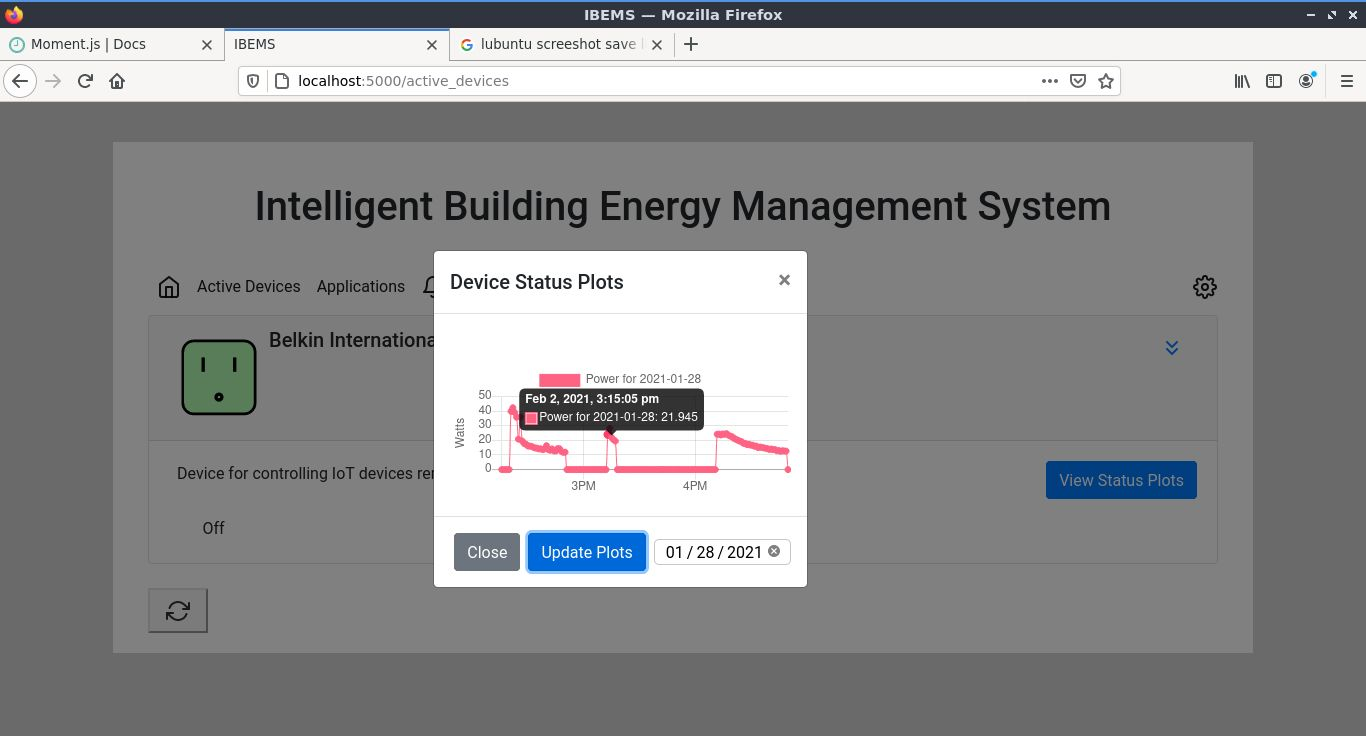
\includegraphics[scale=0.4]{figs/img/badDate.jpg}
\end{figure}   
We solved the issue of the dates being incorrect by updating the javscript code. Next, we are working on calculating the total energy usage over a given day using trapezoidal rule for integration and displaying this value on the webpage. We succesfully developed the algorithm to sum up and calculate the total energy for a given day.

\labday{Thursday, February 4, 2021}
\experiment{Meeting minutes}
Agenda:
\begin{itemize}
\item Code review of method for calculating total energy
\begin{Verbatim}[tabsize=4]
from cassandra.cluster import Cluster
import datetime
import global_settings
import pandas as pd

def totalEnergy(date,deviceID):
    cluster = Cluster()
    session = cluster.connect()
    energySum = 0
    query = ("SELECT time, power FROM " + 
            global_settings.TS_KEYSPACE + "." + 
            "device" + str(deviceID) + 
            " WHERE date = " + "\'" + date + 
            "\'" + " ALLOW FILTERING;")
    result = session.execute(query)
    rows = result.all()
    resultDict = {}
    resultDict['power'] = []
    resultDict['time'] = []
    for row in rows:
        resultDict['power'].append(row.power)
        resultDict['time'].append(
        datetime.datetime.strptime(row.time[:8],"%H:%M:%S"))
    df = pd.DataFrame(data=resultDict)
    df = df.sort_values(by='time')
    resultDict = df.to_dict('list')
    for i in range(len(resultDict['time']) - 1):
        energySum += trapArea(resultDict['time'][i],resultDict['time'][i + 1],
        resultDict['power'][i],resultDict['power'][i+1])
    return energySum

# Trapezoidal rule integration
def trapArea(t1,t2,p1,p2):
    # t1 and t2 are both date time objects 
    dObj = t2 - t1
    return 0.5 * (p1 + p2) * dObj.seconds
\end{Verbatim}
\item Should we prioritize the login feature or the weather service feature?
\item What to include in the poster for the student scholarship expo
\end{itemize}
Minutes
\begin{itemize}
\item Code is fine. We just need to convert to kWh at the end.
\item We should prioritize adding the scheduling feature which we should focus on next week and have done in a month.
\item For now, we should try to get a few more features done before attempting this.
\end{itemize}

\labday{Thursday, February 11, 2021}
\experiment{Meeting minutes}
Agenda
\begin{itemize}
\item Can I (Brian) focus more on the software development portion of the project rather than the EE portion (i.e work on more the web application features than designing the simulation circuits)?
\item What time and day is the scheduling feature due?
\item Should we add a holiday schedule in addition to the weekly schedule for the scheduling feature?
\end{itemize}
Minutes
\begin{itemize}
\item Need the Beaglebone to record power usage
\item Need the scheduling feature to work with the Beaglebone as well
\item The scheduling feature and both devices should be done by end of month (February)
\item We should include a holiday schedule as part of the schedule feature
\item Progress from last week: The motors are working now and Brian has a good start on the scheduling UI.
\end{itemize}

\labday{Thursday, February 18, 2021}
\experiment{Meeting minutes}
Agenda
\begin{itemize}
\item Scheduling feature progress
\begin{itemize}
\item Best way to constantly check for when the status of the device should be updated
\item How to import a python module from a directory one up from the current directory
\item Should we have single agent dedicated for scheduling or all the scheduling functionality implemented in the control agent? 
\item the scheduling agent should be able to send commands to the control agent
\end{itemize}
\item Go over monitoring power usage on the Beaglebone
\begin{itemize}
\item \texttt{rc\_battery\_monitor} command on beaglebone records only voltage of the battery
\item how to calculate the power from this voltage
\item If power isn't possible, could we display percentage of the max voltage of the batteries
\end{itemize}
\end{itemize}
We ended up canceling the meeting this week due to scheduling conflicts.
\medbreak\noindent
I (Brian) ended up testing some of the methods of the new SchedulingAgent to ensure they work. One of the problems I am running into is the issue that I don't know how to delete all rows in a device schedule table in CQL that all have the same day. I was able to get the agent to work for Thursday but soon realized that a table is needed for each device and day. Doing this will require quite a bit of refactoring but at the same time will eliminate hopefully make removing the old schedule a little bit easier. Elliot worked on looking at \texttt{rc\_battery\_monitor} and how to read the voltage from the batteries of the Beaglebone Blue. The issue he is trying to solve is how to read the output from the command into a string and parse it in Python.

\labday{Tuesday, February 23, 2021}
\experiment{Lab work}
BL\\
\smallbreak\noindent
We ended up finishing the scheduling feature for the WeMo, and started work on building support for the BB scheduling. Dr. Miah wants this done by Thursday. We are still trying to figure out how to measure power usage from the beaglebone. One potential option is a USB power meter \footnote{\url{https://www.amazon.com/3-7-30V-Voltage-Multimeter-Current-Voltmeter/dp/B07PWC7YMT}}. However, this USB power meter does not use micro USB.

\medbreak\indent
EW\\
\smallbreak\noindent
The Beaglebone Blue has a USB port, but my concern is that the USB multimeter mentioned above will only measure energy flowing through that USB port and not the entire Beaglebone. We want to know the evergy usage in Watts from the Lipo Battery port on the Beaglebone, but right now we can only measure voltage.

\labday{Wednesday, February 24, 2021}
BL\\
We should do an experiment to do an experiment to figure out the energy of the Beaglebone by looking at current readings.

\labday{Thursday, February 25, 2021}
\experiment{Meeting minutes}
Agenda
\begin{itemize}
\item How should we display the energy in the plot?
\begin{figure}[H]
\centering
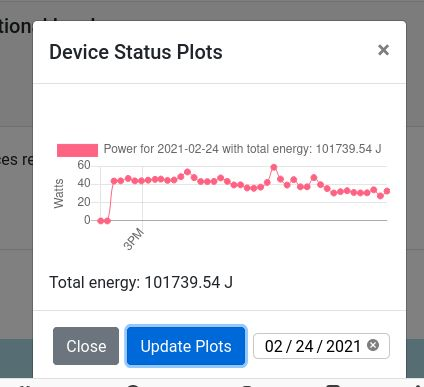
\includegraphics[scale=0.7]{figs/img/plotWithEnergyBelowPlot.jpg}
\end{figure}
\begin{figure}[H]
\centering
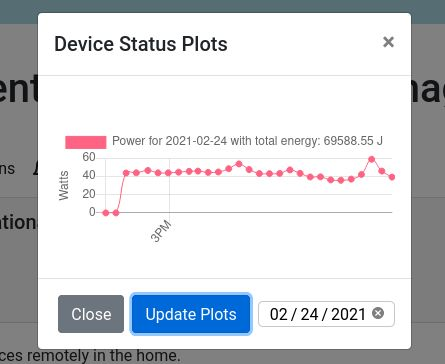
\includegraphics[scale=0.7]{figs/img/plotWithEnergyInTitle.jpg}
\end{figure}
\item Potential Logging feature
\begin{itemize}
\item Agents could log messages to a log file, Python has a built in logging library
\item Should each agent have its own log file or should they all report to the same one
\end{itemize}
\item Best way to measure power from the Beaglebone
\begin{itemize}
\item Use a current sensor breakout board
\item USB power meter, this may not work as the power connector on the Beaglebone uses micro USB
\item Only measure voltage
\end{itemize}
\item I (Brian) have not completed the holiday scheduling feature yet, should we focus on this for the WeMo or rather get the weekly scheduling working with the BB?
\end{itemize}
\experiment{Lab work}
Current values from Beaglebone measured in the lab while motors are running
\begin{itemize}
\item 0.1 duty cycle - roughly 45 mA
\item 0.2 duty cycle - roughly 52 mA
\item 0.3 duty cycle - roughly 59 mA
\item 0.4 duty cycle - roughly 67 mA
\item 0.5 duty cycle - roughly 74 mA
\item 0.6 duty cycle - roughly 80 mA
\item 0.7 duty cycle - roughly 86 mA
\item 0.8 duty cycle - roughly 91 mA
\item 0.9 duty cycle - roughly 95 mA
\item 1.0 duty cycle - roughly 101 mA
\end{itemize}
We merged the Scheduling branch into the master and were able to get the Beaglebone to be controlled through the master branch. Elliot came up with an idea to shut all devices off without a schedule defined for the current time period. So here are the two tasks we want to work on tomorrow:
\begin{itemize}
\item Shut device off if schedule not defined for the current time period
\item Update device tables when loading the applications page
\end{itemize}

\labday{Thursday, March 4, 2021}
\experiment{Meeting minutes}
Agenda
\begin{itemize}
\item What is the minimum amount we need to complete on this project in order for it to be considered finished?
\item How to shutdown the Beaglebone from Python using "sudo shutdown now" from the \texttt{os.system} function or some function defined in the \texttt{subprocess} module
\item Best way to update scheduling data on the applications page when it loads
\item Does it make sense to add buttons to the settings page to alter the sampling rate of the Control Agent and polling rate of the Scheduling Agent?
\item Should we remove links to pages on the site that do not contain any content yet?
\end{itemize}

Minutes
\begin{itemize}
\item Before we graduate, Mr. Matthus will be installing an extra drive in a PC in the senior lab. Ubuntu will be installed on this drive so that the BEMS core can be run from that senior lab PC.
\item TO DO: We need to focus on the beaglebone right now. First: on/off status. Second: Display the battery status (voltage only). On/off status should also be included in the scheduling.
\item We are planning to take a video on Thursday the 11th of all functionality we have on the project so far.
\end{itemize}

Lab Work
\begin{itemize}
\item We found that running this command once will allow any user to shutdown the beaglebone with the command "shutdown now" as opposed to "sudo shutdown now" which required a password. An alternative is the following script:

\begin{Verbatim}
from subprocess import Popen, PIPE

sudo_password = 'temppwd'
command = 'shutdown -h now'.split()

p = Popen(['sudo', '-S'] + command, stdin=PIPE, stderr=PIPE, 
		universal_newlines=True)
sudo_prompt = p.communicate(sudo_password + '\n')[1]
\end{Verbatim}

With this problem solved, the shutdown feature is now complete.
\item Next we got started on displaying the battery voltage from the beaglebone. Getting this voltage is easy enough since existing functions in both C and python exist to retrieve this data. Now it is a matter of sending the voltage reading to the BEMS core.
\end{itemize}

\labday{Thursday, March 18, 2021}
\experiment{Meeting Minutes}
Agenda
\begin{itemize}
\item Abstract for scholarship expo
\item How should the weather data be displayed
\item When do you want the weather feature done by?
\item When do all the bugs need to be fixed?
\end{itemize}

Minutes
\begin{itemize}
\item We will need to add the weather feature before the expo on April 6th:
    \begin{itemize}
    \item Place all data on the home page
    \item Temperature
    \item Humidity
    \item Wind (mph and direction)
    \end{itemize}
\item Put installation steps for BEMS core on the README.md document
\item We need to send LinkedIn requests to Dr. Miah
\item The front end (web pages) need to be prominant (not simple layout)
\item The back end should be reliable (nothing should crash)
\item We sent an email to Mr. Mattus about setting up a PC for our project in the senior lab
\end{itemize}

\labday{Tuesday, March 23, 2021}
\experiment{Lab work}
At the start of the lab, Elliot and I ended up writing a summary for the paper on rEMPy that Dr. Miah found for us. 
\medbreak\noindent
BL\\
At first, I tried installing the rEMpy software on my Windows 10 laptop. However, I wasn't exactly sure how to install everything and some of the dependencies were out of date like Django. Therefore, I wasn't able to get things working. I could try this outside of lab later to get a better idea of what a good project looks like. The next task I worked on was getting a nice page together for the weather data. Most of the web page was built out with a list view showing different quantities like fahrenheit temperature, celcius temperature, wind speed, humidity, and clouds. I went back to installing the software on my Windows laptop to try and get a better idea of how a professional piece of software is made. The software was able to be succesfully run and I created a microgrid. For the last 20 minutes we worked on creating a navbar and restructuring the html files by having a single base.html that the other html files inherit from. We got a basic start on this but need to recolor the navbar.
\end{document} 



%%% Local Variables:
%%% mode: latex
%%% TeX-master: t
%%% End:
